% Options for packages loaded elsewhere
\PassOptionsToPackage{unicode}{hyperref}
\PassOptionsToPackage{hyphens}{url}
%
\documentclass[
  man,floatsintext]{apa7}
\usepackage{amsmath,amssymb}
\usepackage{iftex}
\ifPDFTeX
  \usepackage[T1]{fontenc}
  \usepackage[utf8]{inputenc}
  \usepackage{textcomp} % provide euro and other symbols
\else % if luatex or xetex
  \usepackage{unicode-math} % this also loads fontspec
  \defaultfontfeatures{Scale=MatchLowercase}
  \defaultfontfeatures[\rmfamily]{Ligatures=TeX,Scale=1}
\fi
\usepackage{lmodern}
\ifPDFTeX\else
  % xetex/luatex font selection
\fi
% Use upquote if available, for straight quotes in verbatim environments
\IfFileExists{upquote.sty}{\usepackage{upquote}}{}
\IfFileExists{microtype.sty}{% use microtype if available
  \usepackage[]{microtype}
  \UseMicrotypeSet[protrusion]{basicmath} % disable protrusion for tt fonts
}{}
\makeatletter
\@ifundefined{KOMAClassName}{% if non-KOMA class
  \IfFileExists{parskip.sty}{%
    \usepackage{parskip}
  }{% else
    \setlength{\parindent}{0pt}
    \setlength{\parskip}{6pt plus 2pt minus 1pt}}
}{% if KOMA class
  \KOMAoptions{parskip=half}}
\makeatother
\usepackage{xcolor}
\usepackage{graphicx}
\makeatletter
\def\maxwidth{\ifdim\Gin@nat@width>\linewidth\linewidth\else\Gin@nat@width\fi}
\def\maxheight{\ifdim\Gin@nat@height>\textheight\textheight\else\Gin@nat@height\fi}
\makeatother
% Scale images if necessary, so that they will not overflow the page
% margins by default, and it is still possible to overwrite the defaults
% using explicit options in \includegraphics[width, height, ...]{}
\setkeys{Gin}{width=\maxwidth,height=\maxheight,keepaspectratio}
% Set default figure placement to htbp
\makeatletter
\def\fps@figure{htbp}
\makeatother
\setlength{\emergencystretch}{3em} % prevent overfull lines
\providecommand{\tightlist}{%
  \setlength{\itemsep}{0pt}\setlength{\parskip}{0pt}}
\setcounter{secnumdepth}{-\maxdimen} % remove section numbering
% Make \paragraph and \subparagraph free-standing
\ifx\paragraph\undefined\else
  \let\oldparagraph\paragraph
  \renewcommand{\paragraph}[1]{\oldparagraph{#1}\mbox{}}
\fi
\ifx\subparagraph\undefined\else
  \let\oldsubparagraph\subparagraph
  \renewcommand{\subparagraph}[1]{\oldsubparagraph{#1}\mbox{}}
\fi
\newlength{\cslhangindent}
\setlength{\cslhangindent}{1.5em}
\newlength{\csllabelwidth}
\setlength{\csllabelwidth}{3em}
\newlength{\cslentryspacingunit} % times entry-spacing
\setlength{\cslentryspacingunit}{\parskip}
\newenvironment{CSLReferences}[2] % #1 hanging-ident, #2 entry spacing
 {% don't indent paragraphs
  \setlength{\parindent}{0pt}
  % turn on hanging indent if param 1 is 1
  \ifodd #1
  \let\oldpar\par
  \def\par{\hangindent=\cslhangindent\oldpar}
  \fi
  % set entry spacing
  \setlength{\parskip}{#2\cslentryspacingunit}
 }%
 {}
\usepackage{calc}
\newcommand{\CSLBlock}[1]{#1\hfill\break}
\newcommand{\CSLLeftMargin}[1]{\parbox[t]{\csllabelwidth}{#1}}
\newcommand{\CSLRightInline}[1]{\parbox[t]{\linewidth - \csllabelwidth}{#1}\break}
\newcommand{\CSLIndent}[1]{\hspace{\cslhangindent}#1}
\ifLuaTeX
\usepackage[bidi=basic]{babel}
\else
\usepackage[bidi=default]{babel}
\fi
\babelprovide[main,import]{english}
% get rid of language-specific shorthands (see #6817):
\let\LanguageShortHands\languageshorthands
\def\languageshorthands#1{}
% Manuscript styling
\usepackage{upgreek}
\captionsetup{font=singlespacing,justification=justified}

% Table formatting
\usepackage{longtable}
\usepackage{lscape}
% \usepackage[counterclockwise]{rotating}   % Landscape page setup for large tables
\usepackage{multirow}		% Table styling
\usepackage{tabularx}		% Control Column width
\usepackage[flushleft]{threeparttable}	% Allows for three part tables with a specified notes section
\usepackage{threeparttablex}            % Lets threeparttable work with longtable

% Create new environments so endfloat can handle them
% \newenvironment{ltable}
%   {\begin{landscape}\centering\begin{threeparttable}}
%   {\end{threeparttable}\end{landscape}}
\newenvironment{lltable}{\begin{landscape}\centering\begin{ThreePartTable}}{\end{ThreePartTable}\end{landscape}}

% Enables adjusting longtable caption width to table width
% Solution found at http://golatex.de/longtable-mit-caption-so-breit-wie-die-tabelle-t15767.html
\makeatletter
\newcommand\LastLTentrywidth{1em}
\newlength\longtablewidth
\setlength{\longtablewidth}{1in}
\newcommand{\getlongtablewidth}{\begingroup \ifcsname LT@\roman{LT@tables}\endcsname \global\longtablewidth=0pt \renewcommand{\LT@entry}[2]{\global\advance\longtablewidth by ##2\relax\gdef\LastLTentrywidth{##2}}\@nameuse{LT@\roman{LT@tables}} \fi \endgroup}

% \setlength{\parindent}{0.5in}
% \setlength{\parskip}{0pt plus 0pt minus 0pt}

% Overwrite redefinition of paragraph and subparagraph by the default LaTeX template
% See https://github.com/crsh/papaja/issues/292
\makeatletter
\renewcommand{\paragraph}{\@startsection{paragraph}{4}{\parindent}%
  {0\baselineskip \@plus 0.2ex \@minus 0.2ex}%
  {-1em}%
  {\normalfont\normalsize\bfseries\itshape\typesectitle}}

\renewcommand{\subparagraph}[1]{\@startsection{subparagraph}{5}{1em}%
  {0\baselineskip \@plus 0.2ex \@minus 0.2ex}%
  {-\z@\relax}%
  {\normalfont\normalsize\itshape\hspace{\parindent}{#1}\textit{\addperi}}{\relax}}
\makeatother

\makeatletter
\usepackage{etoolbox}
\patchcmd{\maketitle}
  {\section{\normalfont\normalsize\abstractname}}
  {\section*{\normalfont\normalsize\abstractname}}
  {}{\typeout{Failed to patch abstract.}}
\patchcmd{\maketitle}
  {\section{\protect\normalfont{\@title}}}
  {\section*{\protect\normalfont{\@title}}}
  {}{\typeout{Failed to patch title.}}
\makeatother

\usepackage{xpatch}
\makeatletter
\xapptocmd\appendix
  {\xapptocmd\section
    {\addcontentsline{toc}{section}{\appendixname\ifoneappendix\else~\theappendix\fi\\: #1}}
    {}{\InnerPatchFailed}%
  }
{}{\PatchFailed}
\keywords{filled pauses, disfluencies, non-native-accented speech, feeling of another's knowing\newline\indent Word count: 4774}
\usepackage{lineno}

\linenumbers
\usepackage{csquotes}
\usepackage[titles]{tocloft}
\cftpagenumbersoff{figure}
\renewcommand{\cftfigpresnum}{\itshape\figurename\enspace}
\renewcommand{\cftfigaftersnum}{.\space}
\setlength{\cftfigindent}{0pt}
\setlength{\cftafterloftitleskip}{0pt}
\settowidth{\cftfignumwidth}{Figure 10.\qquad}
\cftpagenumbersoff{table}
\renewcommand{\cfttabpresnum}{\itshape\tablename\enspace}
\renewcommand{\cfttabaftersnum}{.\space}
\setlength{\cfttabindent}{0pt}
\setlength{\cftafterloftitleskip}{0pt}
\settowidth{\cfttabnumwidth}{Table 10.\qquad}
\ifLuaTeX
  \usepackage{selnolig}  % disable illegal ligatures
\fi
\IfFileExists{bookmark.sty}{\usepackage{bookmark}}{\usepackage{hyperref}}
\IfFileExists{xurl.sty}{\usepackage{xurl}}{} % add URL line breaks if available
\urlstyle{same}
\hypersetup{
  pdftitle={Same as always: I suck at titles},
  pdfauthor={Esperanza Badaya1, Robert J. Hartsuiker1, \& Martin Corley2},
  pdflang={en-EN},
  pdfkeywords={filled pauses, disfluencies, non-native-accented speech, feeling of another's knowing},
  hidelinks,
  pdfcreator={LaTeX via pandoc}}

\title{Same as always: I suck at titles}
\author{Esperanza Badaya\textsuperscript{1}, Robert J. Hartsuiker\textsuperscript{1}, \& Martin Corley\textsuperscript{2}}
\date{}


\shorttitle{Horse race experiment}

\authornote{

Correspondence concerning this article should be addressed to Esperanza Badaya. E-mail: \href{mailto:esperanza.badaya@ugent.be}{\nolinkurl{esperanza.badaya@ugent.be}}

}

\affiliation{\vspace{0.5cm}\textsuperscript{1} Ghent University\\\textsuperscript{2} University of Edinburgh}

\abstract{%
Whether an individual is perceived as knowledgeable by others can be biased by several, and potentially irrelevant factors, ranging from the ephemeral (e.g., how speech is produced) to the situational (e.g., who is speaking). The presence of disfluencies, such as filled pauses (e.g., \emph{uh} or \emph{um} in English), elicit evaluations of the speaker as deceitful, less intelligent, or less confident in their knowledge. On the other hand, listeners consider alternative explanations for the speaker to be underinformative: Specifically, non-native speakers are more likely to be forgiven when they fail to be informative. However, whether and how speaker's language profiency affects the interpretation of hesitations and listeners' subsequent behaviour is unclear. In a horse-race betting paradigm, we show that listeners are less likely to follow advice from a speaker who is disfluent, regardless of whether they are disfluent for reasons other than low knowledge. This suggests that previous reported perceptions of knowledgeability elicited explicitly have an impact on how individuals use the information they are given, even in situations when it is not advantageous. Although there is evidence for pragmatic leniance towards non-native speakers, it may be the case that this only applies to failures in language skills that are believed to require high proficiency (e.g., irony), whilst hesitation phenomena may not be subject to such forgiveness. Overall, our results align with a broader body of literature suggesting that the interpretation of hesitation phenomena is not context-dependent.
}



\begin{document}
\maketitle

Impressions of other people arise naturally and automatically (Uleman, Adil Saribay, \& Gonzalez, 2008). Speakers can be evaluated not only by what they say but also by how they say it. For example, vocal features of speech can affect perceptions of confidence and persuasion (Guyer, Fabrigar, \& Vaughan-Johnston, 2019), status and solidarity (Pittam \& Gallois, 1986), or even attractiveness (Feinberg, Jones, Little, Burt, \& Perrett, 2005). One speech feature consistently found to bias evaluations of the speaker is speech fluency. Disfluencies, such as \emph{uh} or \emph{um} in English, can lead to poorer evaluations of the speaker in terms of intelligence (Christenfeld, 1995), competence (Norton-Ford \& Hogan, 1980), and certainty of their own knowledge (Brennan \& Williams, 1995). Interestingly, speech produced with an accent different from one's own - particularly a \emph{foreign} accent - can also elicit negative perceptions of the speaker, including worse evaluations in terms of status, solidarity, and credibility (Gluszek \& Dovidio, 2010; Gluszek, Newheiser, \& Dovidio, 2011; Lev-Ari \& Keysar, 2010; Rakić, Steffens, \& Mummendey, 2011). In this study, however, we explore a rather counterintuitive idea: That the co-presence of these two factors (i.e., (dis)fluency and foreign accents) can diminish the negative impact they have individually. It is important to note that we are not interested whether these cues correlate with a speaker's knowledge or whether listeners believe the speaker to be intentionally misleading: Rather, we are interested in whether, in scenarios where the speaker is expected to be cooperative and knowledgeable, listeners are still biased by irrelevant cues.

There is a growing body of literature showing that certain speech features impact listeners' perceptions of a speaker's knowledgeability. Voices with a slow speech rate, low amplitude, and a large F0 range are less likely to be rated as confident, and produce distinct neural responses (Jiang \& Pell, 2015, 2016b, 2016a). Similarly, prosody guides listeners' evaluations of certainty and honesty cross-linguistically (Goupil, Ponsot, Richardson, Reyes, \& Aucouturier, 2021). These non-verbal qualities of speech may be accompanied by verbal markers of hesitation, such as disfluencies (Grosjean \& Deschamps, 1975; Jiang \& Pell, 2017; Shriberg, Bates, \& Stolcke, 1997; Shriberg \& Lickley, 1993). Brennan and Williams (1995) demonstrated that filled pauses (e.g., uh, mm, or um) impact the perception of speakers' confidence in their knowledge. In their study, participants listened to previously recorded answers to trivia questions (without hearing the questions) and were asked to rate how likely each speaker would be to recognise the correct answer to the question i.e., \emph{feeling of another's knowing}, FOAK. Among the cues that biased participants' assessments were filled pauses: Answers containing a disfluency were more likely to receive lower FOAK ratings, suggesting that filled pauses were taken as reflective of speakers' reduced certainty about their knowledge. In contrast, non-answers (i.e., `I don't know') were more likely to receive a higher FOAK rating if preceded by a filled pause. Brennan and Williams (1995) took this as evidence that listeners are sensitive to the surface form of delivery, and in particular, to the cues displayed by speakers when they do not know (or cannot remember at the moment of being asked) the answer to a question (see also Smith \& Clark, 1993).

Interestingly, speaker identity can itself affect evaluations of both the speaker and the content of speech. In particular, a speaker's nativeness (whether they are producing speech in their first or second language) has been consistently reported to elicit different evaluations. On the one hand, speakers with an accent different from that of the listeners are more likely to be negatively evaluated (e.g., Dragojevic \& Giles, 2016; Gluszek \& Dovidio, 2010). Statements produced with a foreign accent are more likely to receive lower ratings of credibility compared to statements produced with a native accent (Boduch-Grabka \& Lev-Ari, 2021; Lev-Ari \& Keysar, 2010; Barlow et al., 2024; Foucart, Costa, Morís-Fernández, \& Hartsuiker, 2020; Foucart \& Hartsuiker, 2021; Souza \& Markman, 2013; but cf., Stocker, 2017; Wetzel, Zufferey, \& Gygax, 2021). These negative effects of triggered by a speaker's non-nativeness have been accounted for in terms of processing fluency (Lev-Ari \& Keysar, 2010), group membership, and a combination of both (Mai \& Hoffmann, 2013).

On the other hand, there seem to be instances where being a non-native speaker is more advantageous. Fairchild, Mathis, and Papafragou (2020) examined whether and how underinformativeness is interpreted differently as a function of speakers' nativeness. Fairchild et al. (2020) isolated the processing fluency component by presenting written stimuli, so that any differences in attributions were solely guided by speakers' identity. In a series of four experiments, participants read stories where a speaker (native/non-native) described a new invention. Native speakers who were underinformative were more likely to be rated as unwilling to share the information. The same pragmatic failure by a non-native speaker, however, was taken as a sign of inability to produce the necessary information (Exp. 1), even when participants were not explicitly informed that the non-native speaker could experience language difficulties (Exp. 2). Further, this `forgiveness' for underinformative statements had consequences for participants' subsequent behaviours: They were more likely to learn new information from a previously encountered underinformative non-native speaker than from a native speaker (Exp. 3 and 4) (for similar results, see @ Fairchild \& Papafragou, 2018; Lorenzoni, Pagliarini, Vespignani, \& Navarrete, 2022). Interestingly, this pattern of results holds even for auditory stimuli (Ip \& Papafragou, 2022), suggesting that difficulties in comprehending non-native-accented speech alone do not necessarily lead to negative evaluations of the speaker.

One potential explanation is that non-native speakers are evaluated differently from native speakers due to the expectations about their competence. Non-native speakers' accents may invoke stereotypes whereby these speakers are believed to be less competent than native speakers (Fairchild \& Papafragou, 2018; Lev-Ari, 2015). This expectation-based account proposes that stereotypes of non-native speakers' low linguistic competence affect both how their speech is comprehended and interpreted. Specifically, signs that can be attributed to low linguistic competence would be interpreted as such when produced by a non-native speaker and be attributed to other factors when produced by a native speaker. In line with this hypothesis, a speaker's nativeness affects how ironic a statement is perceived to be (Bazzi, Brouwer, \& Foucart, 2022; Caffarra, Michell, \& Martin, 2018) or why non-native speech is processed more shallowly (Hanuíková, Alphen, Goch, \& Weber, 2012; Lev-Ari \& Keysar, 2012).

Interestingly, stereotypes on linguistic competence may also affect how speech is expected to be delivered. For example, a speaker's nativeness has been shown to affect how confident a voice is perceived to be (Caballero \& Pell, 2020; Jiang, Gossack-Keenan, \& Pell, 2019). Given that speakers producing speech in their second language are more disfluent (Bergmann, Sprenger, \& Schmid, 2015; Davies, 2003; Gkalitsiou \& Werle, 2023) and are perceived as such by native listeners (Pinget, Bosker, Quené, \& De Jong, 2014), it could be possible that a speaker's nativeness leads to different interpretations of disfluencies. This would align with findings in the disfluency literature whereby the effects of disfluencies in speech comprehension are dependent on who produces them (Arnold, Kam, \& Tanenhaus, 2007; Barr \& Seyfeddinipur, 2010; Heller, Arnold, Klein, \& Tanenhaus, 2015), including speaker's nativeness (Bosker, Quené, Sanders, \& De Jong, 2014), allegedly because listeners are sensitive to the speaker's mental state and the reasons for being disfluent.

Recently, Matzinger, Pleyer, and Żywiczyński (2023) explored whether listeners' perceptions of why a speaker was disfluent differed for native and non-native speakers. In their study, participants listened to native and non-native speakers answer trivial questions and requests, and were explicitly asked to rate the speaker's knowledge and confidence (for FOAK) and their willingness to grant the request. Crucially, Matzinger et al. (2023) manipulated speakers' fluency by having answers prefaced with either short (200 ms) or long (1200 ms) pauses. For requests, long pauses were less likely to be associated with unwillingness for non-native compared to native speakers. However, FOAK ratings did not differ between speakers: Long pauses produced by either speaker were likely to be taken as reflecting low confidence and low knowledge. Matzinger et al. (2023) attribute this pattern to different conversational contexts: Requests tap into speakers' cooperativeness, and thus in this context, tuning to the interlocutor's mental state and stereotyping might be more relevant than evaluating the speaker's competence (i.e., knowledge).

To date, most experimental evaluations of manner of speech have been explicit. Participants are asked to rate particular traits of speakers on a scale. Further, these ratings are elicited in non-social contexts, where participants do not have anything at stake. Although these experiments demonstrate that listeners show sensitivity to aspects of speech such as fluency and accent when asked to make explicit judgements about the speaker, they may not explain how listeners evaluate speech implicitly, when to do so is consequential.Here, we propose an implicit measurement of listeners' assessments of the speaker's certainty, using a horse-race paradigm. In this task, participants listen to a set of speakers provide descriptions of horses and are asked to distribute virtual tokens as `bets' on each horse's likelihood of winning a putative race. This approach presents two advantages over previous experiments. First, in the horse-race paradigm, participants are not explicitly asked to evaluate a certain trait of the speaker (in this case, how knowledgeable they are). Instead, we take participants' allocations of `betting money' as an indirect measurement of their perceptions of speakers' knowledge. Indeed, pilot studies have shown that individuals are sensitive to this manipulation and that disfluent information leads to smaller bets (Butterworth, 2019). Second, horse races provide a scenario where individuals can make decisions based on what they are told, but the content of speech itself may not be informative for many individuals (in that participants are less familiar with the world of horse racing).

In a pre-registered study, we set up to explore whether and how perceptions of certainty are biased by manner of delivery in the form of fluency and the speaker's identity as conveyed by their accent. We presented participants with recordings of a native and a non-native speaker, each describing two horses, with one description produced fluently and one description produced disfluently. If listeners are sensitive to both local and global causes of hesitations when making judgements about certainty, then disfluent descriptions provided by a native speaker should result in less money bet, reflecting listeners' lower FOAK for the speaker. However, disfluent descriptions provided by a non-native speaker may not impact listeners' betting behaviours, to the extent that they consider the possibility of difficulties in production when assessing the speaker's knowledge. To further control for the potential effects of (non)-nativeness on certainty on its own, we measured participants' language attitudes towards each speaker (see Dragojevic \& Giles, 2016), perceived fluency, accentedness, and comprehensibility of the native and the non-native speaker, as well as the perceived reliability of each speaker. We additionally measured participants' familiarity with and exposure to native and non-native-accented English on a daily basis, to account for the fact that exposure to non-native accents can reduce their negative effects on listeners' judgements (Boduch-Grabka \& Lev-Ari, 2021).

\hypertarget{methods}{%
\section{Methods}\label{methods}}

All experimental stimuli can be found at \url{https://osf.io/zsut7/}.

\hypertarget{participants}{%
\subsection{Participants}\label{participants}}

We conducted a sensitivity power analysis via data simulation following DeBruine and Barr (2021). We explored the required number of participants for a study with a power higher than .8 for the interaction between fluency and speaker identity. We conducted a 1000 simulations per different combinations of the effect size (ranging from small to medium) and the standard deviation of the residuals. In this analysis, we assumed a medium effect size of fluency and no effect of speaker identity. This analysis showed that a sample size of 360 participants ensured enough power to detect a medium or greater effect size.

In our pre-registration, we set that only participants born and raised, and currently residing in the United Kingdom, with English as their first and only language, and with no auditory disorders could partake in the study. Further, we would exclude from analysis data from participants who reported the experiment's aim or manipulation, rated the naturalness of the auditory stimuli (defined as how likely they believed the audios to have been recorded in one go) lower than four, or considered themselves experts in horse races. This meant that we recruited 641 participants for a sample of 360. Participants were recruited via the online platform Prolific, and were reimbursed £1.50 for a 10-minutes experiment.

\hypertarget{visual-stimuli}{%
\subsection{Visual stimuli}\label{visual-stimuli}}

We selected a set of eight images of racehorses from the web. The selected images each featured only one racehorse in the foreground, in motion, ridden by a jockey, and the horses all took up approximately the same proportion of the image. To ensure that the pictures did not bias participants' bets, we recruited ten participants on Prolific, who did not take part in the main study, and asked them to rate on a 10-point scale how likely each horse was to win a hypothetical race and to rank the horses in the order they thought they would cross the finish line, in exchange for £0.45.

A one-way repeated measures ANOVA showed that there were no differences in how likely each horse was thought to be to win a race (F(7) = 0.5, \emph{p} = .83). An ordinal logistic regression showed that none of the horses were more likely to be ranked differently from the others (all \textbar t\textbar{} \textless{} 2). We therefore selected four out of the eight images as visual stimuli.

\hypertarget{auditory-stimuli}{%
\subsection{Auditory stimuli}\label{auditory-stimuli}}

We used four descriptions of racing horses from \emph{The Racing Post}, retrieved on October 2018, originally edited and used by Butterworth (2019). Each passage consisted of three to four sentences describing a horse and its performance in previous races. 30 British English speakers, who did not participate in the final experiment, rated these passages to ensure that all descriptions were perceived as equally likely to describe a winning horse. Participants rated on a 10-point scale how likely they thought each horse was to win a race individually, and then ranked all the horses, in exchange for £0.50.

Based on these results, we further edited the descriptions as some descriptions were more likely to be rated as winning horses. A new sample fo 30 British English speaker rated the edited passages. A one-way repeated measures ANOVA showed no differences in each horse's rated likelihood of winning a race (F(3) = 0.76, \emph{p} = .52), nor in the order in which they were ranked (all \textbar t\textbar{} \textless\$ 2). The final set of descriptions for the experiment can be found in Table \ref{tab:tab-horse-description-text}. Each description was paired with one of the four visual stimuli.

\begin{table}[tbp]

\begin{center}
\begin{threeparttable}

\caption{\label{tab:tab-horse-description-text}Original description of each horse that speakers were asked to memorise and reproduce.}

\begin{tabular}{m{2cm}m{13cm}}
\toprule
Horse & \multicolumn{1}{c}{Description}\\
\midrule
Fire Walker & Fire Walker is looking strong thanks to his come-from-behind success in the Acomb Stakes. The impression given in both runs is that Fire Walker should handle the demands of the extra furlong and Charlie Hills is looking forward to the test. The trainer said ''He's done really well for a little break, his work's been good and I couldn't be more pleased with him''.\\
Silver Sky & Silver Sky, a runner-up of a seven-furlong maiden at Naas on his debut last month, the son of Invincible Spirit ran crack French colt Persian King to a neck in the Group 3 Autumn Stakes over today's trip at Newmarket two weeks ago and his trainer believes he has done well since. O'Brien said ''Silver Sky is a fine big colt and a talented one''.\\
Apocalypse & Apocalypse has put in a string of consistent performances, most recently finishing third to Norway in the Zetland. ''He's had a very solid year'' said trainer Archie Watson. ''He ran a good race in the Zetland, beaten only a length and a quarter, and I think the field here is of a similar level so I'm more than happy for him to take his chance''.\\
Black Blade & Black Blade proved the market all wrong as the complexion of the 6.5-furlong novice race changed dramatically in the final two furlongs, with the Rebel Racing premier-owned newcomer under Tom Queally collaring long-time leaded Monsieur Noir. Spencer said: ''He did it well. He's a nice horse. We always thought had a bright future''.\\
\bottomrule
\end{tabular}

\end{threeparttable}
\end{center}

\end{table}

We then recorded a British English native speaker and a non-native (L1: Italian) English speaker to create the auditory stimuli. Both speakers were female. Passages were recorded one at a time. To elicit naturally disfluent recordings, both speakers were instructed to read the passages silently and then were recorded as they tried to recall the passage from memory. To avoid differences between the descriptions provided by the speakers, they were allowed to look at the descriptions as they spoke if they could not remember the continuation. We edited these recordings using Audacity to ensure that the recordings of each speaker had similar numbers of disfluencies in similar locations, by cross-splicing different recordings (see Table \ref{tab:tab-horse-description-disfluent}). To create the fluent counterpart of each description, filled and mid-utterance silent pauses were excised, and elongations and between-clause silent pauses were reduced using the `Tempo' function. The final auditory experimental stimuli consisted, for each speaker, of two descriptions of each horse (one disfluent, one fluent), resulting in sixteen recordings. Description, fluency, speaker, and order of presentation were counterbalanced in a Latin Square design, resulting in 24 lists.

\begin{table}[tbp]

\begin{center}
\begin{threeparttable}

\caption{\label{tab:tab-horse-description-disfluent}Transcription of the disfluent horse descriptions.}

\begin{tabular}{m{2cm}m{13cm}}
\toprule
Horse & \multicolumn{1}{c}{Description}\\
\midrule
Fire Walker & FP-um Fire Walker is looking SP strong thanks to his (elongation) SP come-from-behind success SP FP-er in the Acomb Stakes. FP-um The (elongation) impression given SP in both runs FP-uh is that Fire Walker should SP handle the demands of SP the extra furlong and FP-uh Charlie Hills is looking forward to the test. The trainer said ''He's done (elongation) FP-um really well for a little break, FP-uh his work's been good and I couldn't be more pleased with him''.\\
Silver Sky & Silver Sky, FP-uh a runner-up of -a seven-furlong maiden at Naas on his (elongation) debut last month. FP-uh The son of Invincible Spirit SP\ \ ran (elongation) crack French colt Persian King\ \  to a neck in the FP-uh\ \ Group 3 Autumn Stakes. over today's trip at Newmarket two weeks ago FP-uh and his trainer believes he has done well since. O'Brien said FP-uh ''Silver Sky is a fine big colt and a talented one''.\\
Apocalypse & FP Apocalypse has put in a (elongation-ish) string SP of consistent performances, FP most recently finishing third to SP Norway in the Zetland. FP ''He's had a very solid year'' said trainer SP FP Archie Watson. ''He ran a SP good race in the Zetland, SP FP SP beaten only a length and a quarter, and I think the field here SP is of a similar level so I'm- I'm more than happy for him to (elongation-ish) take his chance''.\\
Black Blade & FP-um Black SP Blade proved SP FP-uh the market all wrong as the complexion SP of the 6.5 furlong SP novice SP race FP-um changed dramatically in SP the final two furlong. SP FP-uh with the\ \ Rebel Racing SP premier-owned SP newcomer under Tom SP Queally FP-um SP collaring long-time leaded Monsieur Noir. FP-uh Spencer said: ''He did it well. FP-uh He's a nice horse. FP-uh We always thought he had a bright future''.\\
\bottomrule
\end{tabular}

\end{threeparttable}
\end{center}

\end{table}

To ensure that the resulting descriptions were perceived to be natural (i.e., our edited `fluent' audios were not clearly edited) and that they were perceived as differing in fluency (i.e., disfluent and `fluent' versions were distinguishable), we validated them in a sample of 48 British English participants, who did not take further part in the study. Participants were allocated to one of the 24 experimental lists, to ensure that our validation procedure was similar to how participants encountered stimuli in the actual experiment. Following Bosker, Quené, Sanders, and De Jong (2014) procedure, participants were asked to rate each audio's fluency on a scale from 1 to 9 (1: not fluent at all, 9: very fluent). We instructed participants to rate fluency by considering silent and filled pauses, speed of speech, and repairs, and to ignore speakers' accents and the content of their speech. Participants additionally rated on a 9-point scale each recording's naturalness (defined as how likely it was that the audio had been recorded in one go; 1: not unlikely at all; 9: very likely), and accentedness (while ignoring the perceived speaker's proficiency in the language; 1: not accented at all, 9: very accented). We additionally asked participants to guess the speakers' country of origin. At the end of the task, participants were further asked how often they interacted with native and non-native English speakers (on a 9-point scale, 1: never, 9: always) and were allowed to report if they noticed anything odd in the auditory stimuli.

\begin{table}[tbp]

\begin{center}
\begin{threeparttable}

\caption{\label{tab:tab-results-validation}Mean (standard deviation) ratings of native and non-native speakers’ fluent and disfluent
recordings for fluency, naturalness, and accentedness, on a 9-point scale where lower values indicate
less fluent, less natural, and less accent respectively.}

\begin{tabular}{lllll}
\toprule
Speaker & \multicolumn{1}{c}{Delivery} & \multicolumn{1}{c}{Fluency} & \multicolumn{1}{c}{Naturalness} & \multicolumn{1}{c}{Accentedness}\\
\midrule
Native Speaker & Fluent & 7.62 (1.59) & 5.44 (2.62) & 4.38 (2.22)\\
 & Disfluent & 6.44 (2.36) & 5.73 (2.57) & 4 (1.97)\\
Non-native Speaker & Fluent & 6.25 (1.73) & 5.94 (1.83) & 7.02 (1.59)\\
 & Disfluent & 5.21 (1.75) & 5.83 (1.99) & 7.17 (1.51)\\
\bottomrule
\end{tabular}

\end{threeparttable}
\end{center}

\end{table}

Table \ref{tab:tab-results-validation} shows the means (and standard deviations) of participants' ratings of fluency, naturalness, and accentedness. A linear mixed model for fluency ratings with fixed effects of fluency (treatment-coded, reference: fluent), speaker's linguistic background (treatment-coded, reference: native speaker), and their interaction, with random intercepts by participant and by horse description showed that fluency ratings differed significantly for the fluent and disfluent conditions (\(\hat{\beta} = -1.19\), 95\% CI \([-1.79, -0.58]\), \(t = -3.84\)). The non-native speaker was perceived as more disfluent than the native speaker (\(\hat{\beta} = -1.37\), 95\% CI \([-1.97, -0.78]\), \(t = -4.51\)), in line with previous findings (Bosker, Quené, Sanders, \& Jong, 2014; Pinget et al., 2014), but the interaction between the two variables was not significant (\(\hat{\beta} = 0.15\), 95\% CI \([-0.49, 0.78]\), \(t = 0.45\)). An identical model for naturalness ratings showed no significant differences by fluency (\(\hat{\beta} = 0.29\), 95\% CI \([-0.52, 1.11]\), \(t = 0.70\)), speaker's linguistic background (\(\hat{\beta} = 0.50\), 95\% CI \([-0.27, 1.27]\), \(t = 1.27\)) or their interaction (\(\hat{\beta} = -0.40\), 95\% CI \([-1.49, 0.70]\), \(t = -0.71\)).

\hypertarget{procedure}{%
\section{Procedure}\label{procedure}}

Stimuli were presented using JsPsych (Leeuw, Gilbert, \& Luchterhandt, 2023), hosted on MindProbe (via JATOS, Lange, Kühn, \& Filevich, 2015). The task began with a cover story introducing two horse racing tipsters. Participants were told the tipsters would provide information about the four most popular horses competing in an upcoming race at Musselburgh Racecourse (Edinburgh). The cover story explained that the two tipsters were well-known experts in the field, and added that one of the speakers was a non-native English speaker (without specifying the nationality of either speaker), introducing the element of the speakers' linguistic backgrounds as well as the factor of competence.

At the beginning of the experiment, participants were shown four pictures of the horses that they had been told would take part in the race, alongside their names. Participants were instructed to distribute one-hundred pounds in betting money across the four horses based on the likelihood they thought each horse had of winning: They could split the bets as they wished, and they did not have to spend all the money. Each participant was randomly assigned to one out of 24 groups, so that they would listen to each speaker twice, one in each fluency level. The order in which horses were presented was randomised. In each trial, participants listened to one speaker described a given horse's performance. Once the playback stopped, participants were asked to place a bet by typing a number on a web form. Participants could only move to the next horse's description once they had placed a bet. Participants were allowed to modify their previous bets every time they heard a new description. If the sum of bets made at any point was more than the allotted maximum, they were asked to re-distribute their bets until the total was below one-hundred pounds.

After the betting round was complete, participants completed a questionnaire similar to that of Foucart et al. (2020) to measure their language attitudes towards the native and the non-native speaker. For each speaker, participants answered six questions measuring affect (three questions for negative affect and three questions for positive affect), five questions measuring solidarity, five questions measuring status, and one question each for comprehensibility, accentedness, fluency, and trustworthiness. Each question used a 9-point scale. Participants first answered questions about, at random, the native or non-native speaker, with the order of presentation of dimensions being randomised. They then answered the same questions for the remaining speaker. We also asked participants to guess the countries of origin of our native and non-native speakers, and from which speaker they would like to learn about horse races in the future. Additional questions included ratings on a 9-point scale of how natural the audio sounded (1: unnatural, edited; 9: natural, unedited), and two questions measuring participants' exposure to native and non-native accented English (1: never; 9: always). Likewise, we measured participants' previous experience with betting and their perceived knowledge of horse races (two questions: Whether they had bet on horse races in the past, and to rate on a 5-point scale, from `Strongly disagree' to `Strongly agree', how closely they identified with the statement `I am an expert on horse races'). Finally, we included an open-ended question for participants to report what guided their decision-making, as well as their perception of the experiment's aim.

\hypertarget{results}{%
\section{Results}\label{results}}

All data pre-processing and analyses were carried out in R version 4.4.1 (R Core Team, 2024), using the packages \emph{tidyverse} version 2.0.0 (Wickham et al., 2019), \emph{ggplot} version 3.5.1 (Wickham, 2016), and \emph{wesanderson} version for data wrangling and visualization. \emph{lme4} version 1.1-35.5 (Bates, Mächler, Bolker, \& Walker, 2015) was used for data analysis, and \emph{papaja} version 0.1.2 (Aust \& Barth, 2023) for manuscript write-up. Scripts can be found at \url{https://osf.io/zsut7/}

\hypertarget{pre-registered-analyses}{%
\subsection{Pre-registered analyses}\label{pre-registered-analyses}}

\hypertarget{betting-behaviour}{%
\subsubsection{Betting behaviour}\label{betting-behaviour}}

Table \ref{tab:tab-dist-money} and Figure \ref{fig:fig1} show the mean amount of money bet per speaker and fluency condition. On average, participants bet £25 on each horse. This distribution suggests that participants followed a rational behaviour: Given their lack of expertise, they distributed the one hundred pounds equally. However, disfluent instructions seem to lower the amount of money bet.

\begin{table}[tbp]

\begin{center}
\begin{threeparttable}

\caption{\label{tab:tab-dist-money}Mean (standard deviation) of money bet by manner of delivery and speaker’s linguistic
background.}

\begin{tabular}{lll}
\toprule
Speaker & \multicolumn{1}{c}{Delivery} & \multicolumn{1}{c}{Money bet}\\
\midrule
Native & Fluent & 24.24 (13.92)\\
 & Disfluent & 20.66 (12.23)\\
Non-native & Fluent & 24.15 (13.61)\\
 & Disfluent & 22.31 (13.81)\\
\bottomrule
\end{tabular}

\end{threeparttable}
\end{center}

\end{table}

\begin{figure}[H]

{\centering 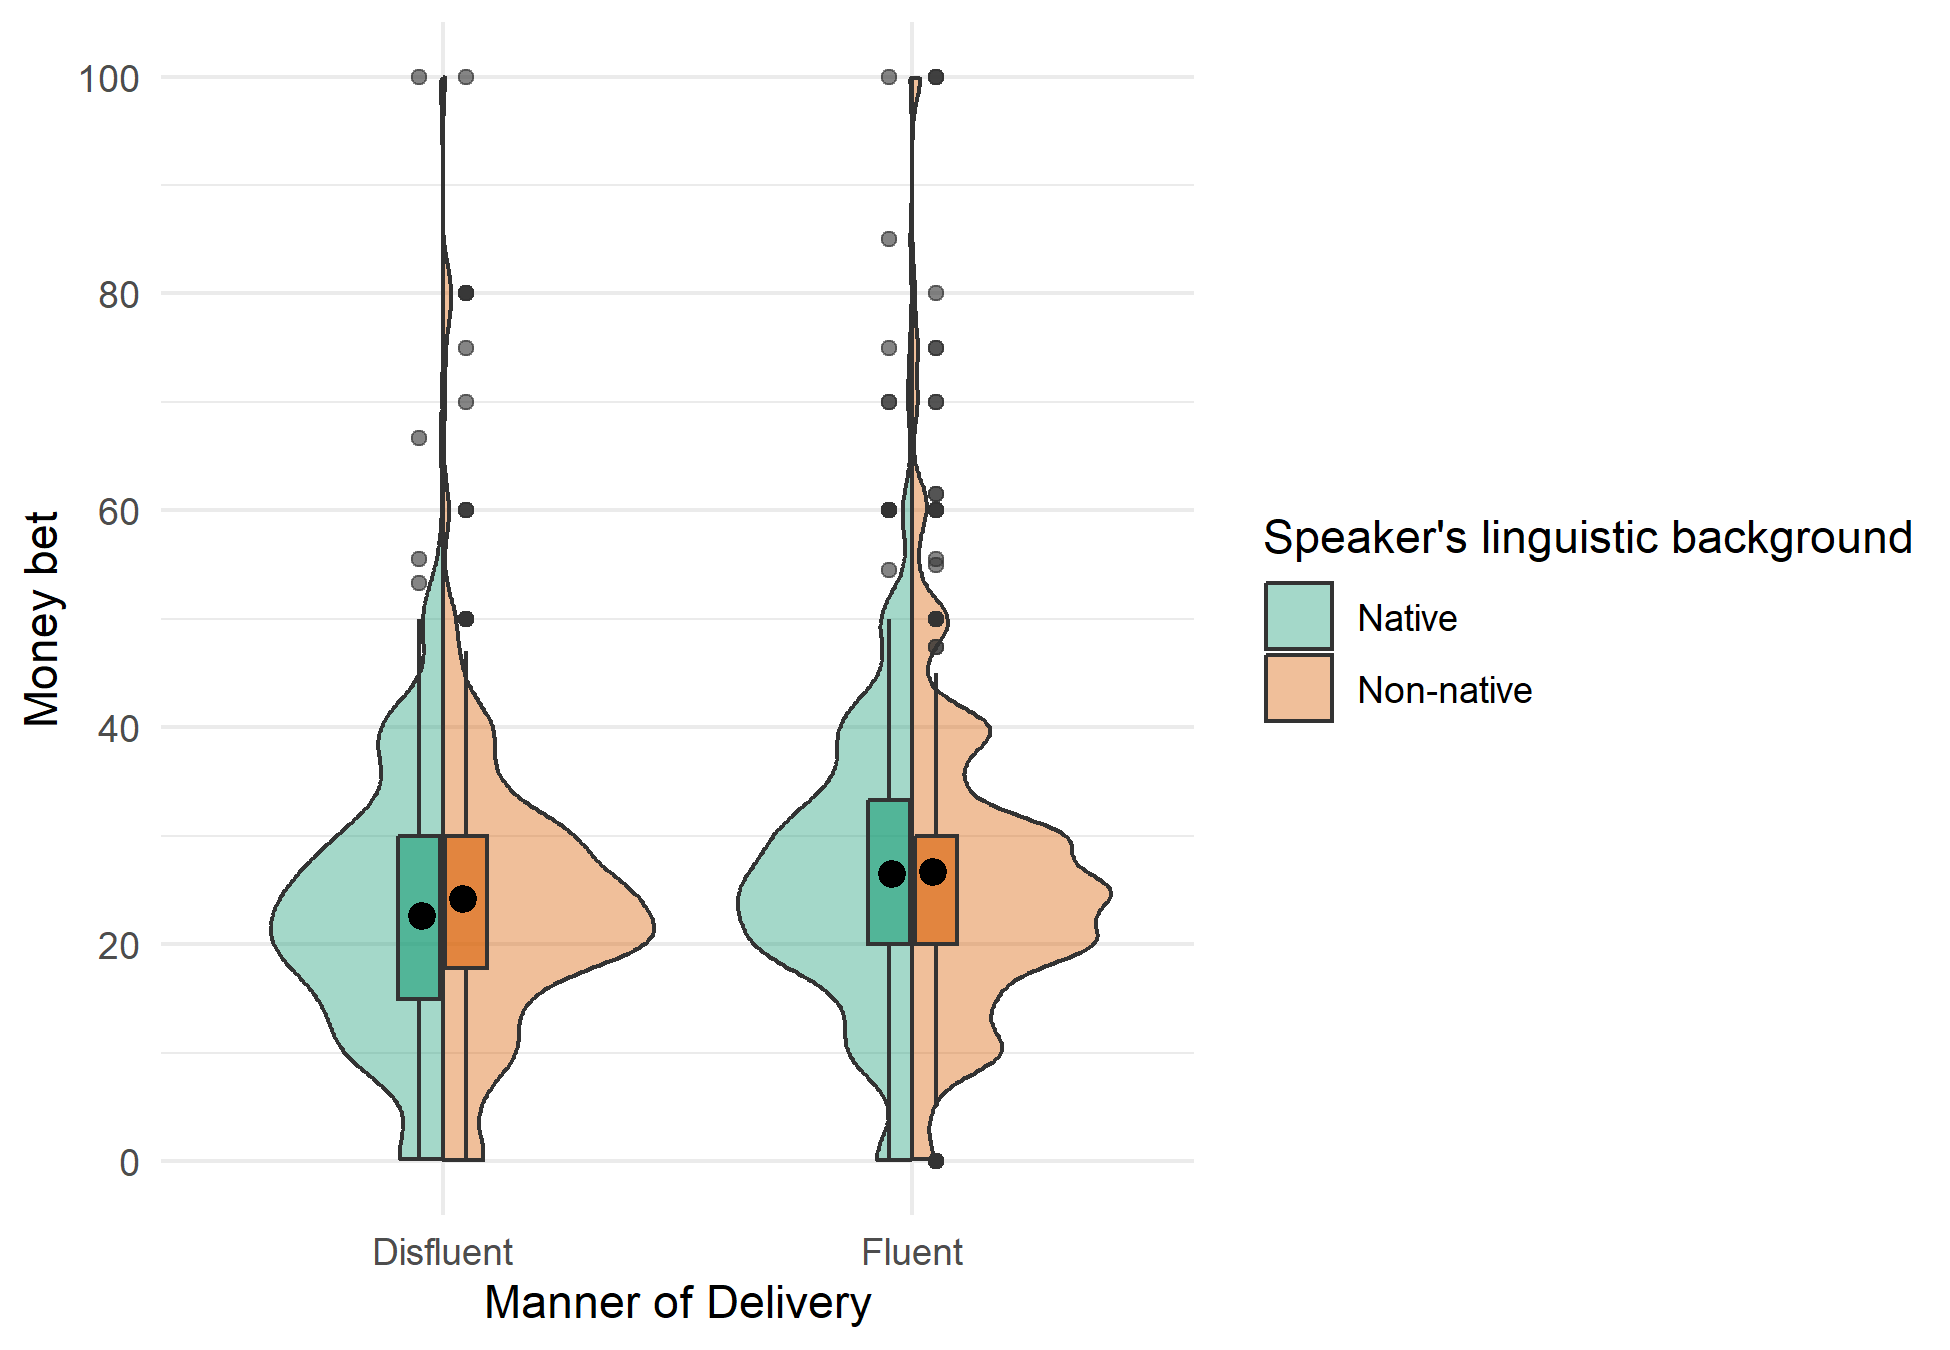
\includegraphics[width=0.9\linewidth,]{manuscript_eb_files/figure-latex/fig1-1} 

}

\caption{Money distribution by manner of delivery (fluent/disfluent) and speaker (green: native/orange: non-native).}\label{fig:fig1}
\end{figure}

We modelled participants' betting behaviour in a linear mixed model. We modelled money bet on each horse, taken from the final amounts submitted in the experiment, after all four descriptions had been heard and valid responses (summing to at most 100 pounds) had been recorded. The model included fixed effects of fluency (sum-coded; fluent coded as -0.5, disfluent as +0.5), speaker's linguistic background (sum-coded, native coded as -0.5; non-native coded as +0.5), and their interaction. The maximal model (Barr, Levy, Scheepers, \& Tily, 2013), with random intercepts by-participant and by-item, with random slopes for fluency and speaker's linguistic background by-participant, and for fluency by-item, failed to converge. We first dropped the random intercept by-participant, as most participants used all the money and thus there was no variance in their intercept. The final model included a random intercept by-item. Results were deemed significant at \textbar t\textbar{} \textgreater{} 2 (Baayen, 2008).

Our model showed a main effect of fluency, whereby participants placed lower bets following disfluent descriptions compared to their fluent counterparts (\(\hat{\beta} = -2.71\), 95\% CI \([-4.04, -1.38]\), \(t = -3.99\)). There was no main effect of speaker (\(\hat{\beta} = 0.78\), 95\% CI \([-0.55, 2.11]\), \(t = 1.15\)) and importantly, no interaction between delivery and speaker (\(\hat{\beta} = 1.74\), 95\% CI \([-0.92, 4.40]\), \(t = 1.28\))\footnote{An identical model including excluded participants showed a main effect of fluency (\(\hat{\beta} = -2.71\), 95\% CI \([-4.04, -1.38]\), \(t = -3.99\)), and no other significances (for speaker, \(\hat{\beta} = 0.78\), 95\% CI \([-0.55, 2.11]\), \(t = 1.15\); for the interaction \(\hat{\beta} = 1.74\), 95\% CI \([-0.92, 4.40]\), \(t = 1.28\))}.

\hypertarget{language-attitudes}{%
\subsubsection{Language attitudes}\label{language-attitudes}}

Table \ref{tab:tab5} depicts the mean (and standard deviation) of ratings in each of the measures of interest by speaker's linguistic background. Constructs measured with more than one question (affect, status, solidarity) were obtained by calculating the average score. For the \emph{Affect} dimension, we reverse-scored items measuring negative affect. Cronbach's alpha showed that the scores for these attitudes were reliable (\(\alpha_{affect}\) = 0.80, \(\alpha_{status}\) = 0.93, \(\alpha_{solidarity}\) = 0.87). We explored differences between the native and the non-native speaker's evaluations in these three social dimensions as well as on Comprehensibility, Accentedness, and Trustworthiness via paired t-test using Bonferroni correction for \emph{p} values.

\begin{table}[tbp]

\begin{center}
\begin{threeparttable}

\caption{\label{tab:tab5}Average score (and standard deviation) in each dimension by speaker.}

\begin{tabular}{lll}
\toprule
Dimension & \multicolumn{1}{c}{Native Speaker} & \multicolumn{1}{c}{Non-native Speaker}\\
\midrule
Comprehensibility & 7.62 (1.57) & 5.51 (2.14)\\
Accentedness & 5.46 (2.1) & 6.84 (1.37)\\
Affect & 5.77 (1.49) & 6.05 (1.32)\\
Status & 5.95 (1.52) & 6.43 (1.31)\\
Solidarity & 5.67 (1.48) & 6.41 (1.24)\\
Trustworthy & 6 (1.61) & 6.36 (1.41)\\
\bottomrule
\end{tabular}

\end{threeparttable}
\end{center}

\end{table}

\begin{table}[tbp]

\begin{center}
\begin{threeparttable}

\caption{\label{tab:tab6}Paired t test for each dimension between speakers.}

\begin{tabular}{llll}
\toprule
Dimension & \multicolumn{1}{c}{t(359)} & \multicolumn{1}{c}{95\% CI} & \multicolumn{1}{c}{d}\\
\midrule
Comprehensibility & 15.99 & {}[1.85, 2.36] & 2.11\\
Accent & -11.51 & {}[-1.62, -1.15] & -1.39\\
Affect & -3.54 & {}[-0.44, -0.13] & -0.29\\
Status & -6.55 & {}[-0.62, -0.33] & -0.48\\
Solidarity & -9.63 & {}[-0.89, -0.59] & -0.74\\
Trustworthy & -4.12 & {}[-0.53, -0.19] & -0.36\\
\bottomrule
\end{tabular}

\end{threeparttable}
\end{center}

\end{table}

Analyses showed that speakers were rared differently across all six dimensions (see Table \ref{tab:tab6}). The largest differences were, unsurprisingly, in comprehensibility and accentedness, where the non-native speaker received lower ratings.

Following our pre-registered analysis, we included these six variables in our previous model to explore whether speakers' evaluations could further explain participants' betting behaviours. This second model improved model fit (\(\chi^2\)(6) = 19.46, \emph{p} \textless{} .01). Besides a main effect of manner of delivery (\(\hat{\beta} = -2.71\), 95\% CI \([-4.03, -1.39]\), \(t = -4.02\)), the model showed an effect of affect, whereby higher ratings of affect were more likely to yield higher bettings (\(\hat{\beta} = 0.81\), 95\% CI \([0.14, 1.49]\), \(t = 2.35\))

\hypertarget{exploratory-analysis}{%
\subsection{Exploratory analysis}\label{exploratory-analysis}}

We additionally explored participants' preferences to learn from either speaker in the future. 206 participants reported they would prefer to learn from the native spaker, and 154 preferred the non-native speaker. A \(\chi^2\) test of goodness of fit showed that there was a significant difference in participants' preferences (\(\chi^2\)(1) = 7.51, \emph{p} \textless{} .01).

\hypertarget{discussion}{%
\section{Discussion}\label{discussion}}

Listeners can attribute a speaker knowledgeability based on a range of cues, such as voice pitch or amplitude. Speech (dis)fluency has been previously shown to impact how confident in their knowledge a speaker is judged to be (Brennan \& Williams, 1995). However, speakers can be disfluent for reasons other than (un)confidence: For example, speaking in one's second language is also associated with an increase in disfluencies (De Jong, Groenhout, Schoonen, \& Hulstijn, 2015; Derwing, Munro, Thomson, \& Rossiter, 2009). In fact, it has been proposed that second language speakers are stereotyped and thus expected to display low linguistic performance (Lev-Ari, 2015), which consequently leads native listeners to ``forgive'' what otherwise would be lead to a negative evaluation (Fairchild et al., 2020; Lorenzoni et al., 2022). In the present experiment, we explored whether attributions of (un)knowledgeability as a function of the speaker's nativeness, and if those affected listeners' subsequent behaviours in a task where participants had to place bets on horse. Our findings suggest that manner of delivery, in the form of fluency, was the sole factor that guided participants' behavior: Disfluent descriptions yielded lower bets, regardless of who was speaking.

The pattern found aligns with the idea that listeners are sensitive to how an utterance is produced (Brennan \& Williams, 1995). Descriptions that included hesitation phenomena, in the form of filled pauses, led to smaller bets compared to their fluent counterparts. This aligns with Brennan and Williams (1995) findings wherein listeners were less likely to attribute confidence in their knowledge to a speaker when their answers included hesitation phenomena (i.e., Feeling of Another's Knowing). Brennan and Williams (1995) attributed participants' ratings to inferences made about the speaker's mental state - specifically, inferences about the degree of confidence a speaker has in their knowledge. In our experiment, since participants have little a priori knowledge that can guide their betting behaviour, and because the utterance is semantically and acoustically identical apart from the excision of disfluencies, an inference about a speaker's confidence based on those disfluencies is an important potential determinant of participants' decisions.

This inference explanation would predict that listeners would forgive foreign disfluencies, in line with the expectations-based account. While previous research has reported that whether a filled pause affects processes involved in speech comprehension depending on speaker identity (e.g., Bosker, Quené, Sanders, \& De Jong, 2014), recent studies have failed to find this effect when it comes to speaker's attributions (Matzinger et al., 2023). In our experiment, participants distributed money similarly when either speaker provided disfluent descriptions, suggesting that listeners did not weigh in our (non-native) speaker's identity to interpret the disfluency. This is particularly remarkable given that in our post-experimental questionnaire, the native speaker was more likely to be chosen as someone participants would like to learn from about horse races in the future. One possibility for this lack of interaction has to do with the fact that our non-native speaker was introduced as a knowledgeable tipster. This introduction of the speaker as an authoritative figure may have overridden any other features of their identity, including their non-native speaker identity. Indeed, beliefs about a speaker's expertise have been shown to guide perceptions of their certainty (Mol, Kuhlen, Van der Steen, \& Obbens, 2013). Considering the language attitudes triggered by both accents, the difference in speaker preference may more likely reflect the ease of comprehending the native speaker, rather than an implicit negative bias towards the non-native speaker, and particularly, a diminished perception of competence for non-native speakers.

The experiment here also introduced a novel approach to measuring how certain the speaker is perceived. While previous studies had participants explicitly rate a speaker on different dimensions (e.g., knowledgeability, trust) in non-social contexts, the present study offers a new venue to explore how different factors bias individuals' evaluations indirectly, as well as the implications of those evaluations. However, a potential shortcoming of our design has to do with how people approached the betting system. Because of the nature of the task, in that we tested participants with no prior knowledge of horse races, our participants behaved rationally: The vast majority employed the hundred pounds allocated and distributed them fairly rationally in a way that maximizes their chances of winning (i.e., around £25 per horse). It is, therefore, possible that in situations of less uncertainty (e.g., a scenario where individuals have more knowledge) or where they are rewarded for allocating money to the winning horse, how the speaker is perceived may yield a larger effect on participants' behaviours.

\newpage

\hypertarget{references}{%
\section{References}\label{references}}

\hypertarget{refs}{}
\begin{CSLReferences}{1}{0}
\leavevmode\vadjust pre{\hypertarget{ref-arnoldetal2007}{}}%
Arnold, J. E., Kam, C. L. H., \& Tanenhaus, M. K. (2007). If you say thee uh you are describing something hard: The on-line attribution of disfluency during reference comprehension. \emph{Journal of Experimental Psychology: Learning, Memory, and Cognition}, \emph{33}(5), 914--930. \url{https://doi.org/10.1037/0278-7393.33.5.914}

\leavevmode\vadjust pre{\hypertarget{ref-R-papaja}{}}%
Aust, F., \& Barth, M. (2023). \emph{{papaja}: {Prepare} reproducible {APA} journal articles with {R Markdown}}. Retrieved from \url{https://github.com/crsh/papaja}

\leavevmode\vadjust pre{\hypertarget{ref-baayen2008}{}}%
Baayen, R. H. (2008). \emph{Analyzing linguistic data: A practical introduction to statistics using r}. Cambridge University Press. \url{https://doi.org/10.1017/CBO9780511801686}

\leavevmode\vadjust pre{\hypertarget{ref-barlowetal2024}{}}%
Barlow, S., Beardsley, G., Bsharah, Z., Crofts, R., De La Rosa, C., Gutierrez, A., et al.others. (2024). The effects of exposure and explicit stereotypes on veracity judgments of polish-accented english speech: A preregistered close replication and extension of boduch-grabka \& lev-ari (2021). \emph{Studies in Second Language Acquisition}, 1--17.

\leavevmode\vadjust pre{\hypertarget{ref-barretal2013}{}}%
Barr, D. J., Levy, R., Scheepers, C., \& Tily, H. J. (2013). Random effects structure for confirmatory hypothesis testing: Keep it maximal. \emph{Journal of Memory and Language}, \emph{68}(3), 255--278. \url{https://doi.org/10.1016/j.jml.2012.11.001}

\leavevmode\vadjust pre{\hypertarget{ref-barrseyfeddinipur2010}{}}%
Barr, D. J., \& Seyfeddinipur, M. (2010). The role of fillers in listener attributions for speaker disfluency. \emph{Language and Cognitive Processes}, \emph{25}(4), 441--455.

\leavevmode\vadjust pre{\hypertarget{ref-lme4}{}}%
Bates, D., Mächler, M., Bolker, B., \& Walker, S. (2015). Fitting linear mixed-effects models using {lme4}. \emph{Journal of Statistical Software}, \emph{67}(1), 1--48. \url{https://doi.org/10.18637/jss.v067.i01}

\leavevmode\vadjust pre{\hypertarget{ref-bazzietal2022}{}}%
Bazzi, L., Brouwer, S., \& Foucart, A. (2022). The impact of foreign accent on irony and its consequences on social interaction. \emph{Journal of Multilingual and Multicultural Development}, 1--13.

\leavevmode\vadjust pre{\hypertarget{ref-bergmannetal2015}{}}%
Bergmann, C., Sprenger, S. A., \& Schmid, M. S. (2015). The impact of language co-activation on {L1} and {L2} speech fluency. \emph{Acta {Psychologica}}, \emph{161}, 25--35.

\leavevmode\vadjust pre{\hypertarget{ref-boduchlevari2021}{}}%
Boduch-Grabka, K., \& Lev-Ari, S. (2021). Exposing individuals to foreign accent increases their trust in what nonnative speakers say. \emph{Cognitive Science}, \emph{45}(11), e13064. \url{https://doi.org/10.1111/cogs.13064}

\leavevmode\vadjust pre{\hypertarget{ref-boskeretal2014}{}}%
Bosker, H. R., Quené, H., Sanders, T., \& De Jong, N. H. (2014). Native `um's elicit prediction of low-frequency referents, but non-native `um's do not. \emph{Journal of Memory and Language}, \emph{75}, 104--116. \url{https://doi.org/10.1016/j.jml.2014.05.004}

\leavevmode\vadjust pre{\hypertarget{ref-boskeretal2014b}{}}%
Bosker, H. R., Quené, H., Sanders, T., \& Jong, N. H. de. (2014). The perception of fluency in native and nonnative speech. \emph{Lang. Learn.}, \emph{64}(3), 579--614. \url{https://doi.org/10.1111/lang.12067}

\leavevmode\vadjust pre{\hypertarget{ref-brennanwilliams1995}{}}%
Brennan, S. E., \& Williams, M. (1995). The feeling of another's knowing: Prosody and filled pauses as cues to listeners about the metacognitive states of speakers. \emph{Journal of Memory and Language}, \emph{34}(3), 383--398.

\leavevmode\vadjust pre{\hypertarget{ref-butterworth2019}{}}%
Butterworth, H. (2019). \emph{How much do they, um, know?: Disfluencies in speech as cues to speakers' knowledge.} University of Edinburgh.

\leavevmode\vadjust pre{\hypertarget{ref-caballeropell2020}{}}%
Caballero, J. A., \& Pell, M. D. (2020). Implicit effects of speaker accents and vocally-expressed confidence on decisions to trust. \emph{Decision}, \emph{7}(4), 314. \url{https://doi.org/10.1037/dec0000140}

\leavevmode\vadjust pre{\hypertarget{ref-caffarraetal2018}{}}%
Caffarra, S., Michell, E., \& Martin, C. D. (2018). The impact of foreign accent on irony interpretation. \emph{{PLoS} One}, \emph{13}(8), e0200939.

\leavevmode\vadjust pre{\hypertarget{ref-christenfeld1995}{}}%
Christenfeld, N. (1995). Does it hurt to say um? \emph{Journal of Nonverbal Behavior}, \emph{19}, 171--186.

\leavevmode\vadjust pre{\hypertarget{ref-davies2003}{}}%
Davies, A. (2003). \emph{The native speaker: Myth and reality} (Vol. 38). Multilingual matters. \url{https://doi.org/10.21832/9781853596247}

\leavevmode\vadjust pre{\hypertarget{ref-dejongetal2015}{}}%
De Jong, N. H., Groenhout, R., Schoonen, R., \& Hulstijn, J. H. (2015). Second language fluency: Speaking style or proficiency? Correcting measures of second language fluency for first language behavior. \emph{Applied Psycholinguistics}, \emph{36}(2), 223--243.

\leavevmode\vadjust pre{\hypertarget{ref-debruinebarr2021}{}}%
DeBruine, L. M., \& Barr, D. J. (2021). Understanding mixed-effects models through data simulation. \emph{Advances in Methods and Practices in Psychological Science}, \emph{4}(1), 2515245920965119. \url{https://doi.org/10.1177/251524592096511}

\leavevmode\vadjust pre{\hypertarget{ref-derwingetal2009}{}}%
Derwing, T. M., Munro, M. J., Thomson, R. I., \& Rossiter, M. J. (2009). The relationship between L1 fluency and L2 fluency development. \emph{Studies in Second Language Acquisition}, \emph{31}(4), 533--557.

\leavevmode\vadjust pre{\hypertarget{ref-dragojevicgiles2016}{}}%
Dragojevic, M., \& Giles, H. (2016). I don't like you because you're hard to understand: The role of processing fluency in the language attitudes process. \emph{Human Communication Research}, \emph{42}(3), 396--420. \url{https://doi.org/10.1111/hcre.12079}

\leavevmode\vadjust pre{\hypertarget{ref-fairchildetal2020}{}}%
Fairchild, S., Mathis, A., \& Papafragou, A. (2020). Pragmatics and social meaning: Understanding under-informativeness in native and non-native speakers. \emph{Cognition}, \emph{200}, 104171.

\leavevmode\vadjust pre{\hypertarget{ref-fairchildpapafragou2018}{}}%
Fairchild, S., \& Papafragou, A. (2018). Sins of omission are more likely to be forgiven in non-native speakers. \emph{Cognition}, \emph{181}, 80--92.

\leavevmode\vadjust pre{\hypertarget{ref-feinbergetal2005}{}}%
Feinberg, D. R., Jones, B. C., Little, A. C., Burt, D. M., \& Perrett, D. I. (2005). Manipulations of fundamental and formant frequencies influence the attractiveness of human male voices. \emph{Animal Behaviour}, \emph{69}(3), 561--568.

\leavevmode\vadjust pre{\hypertarget{ref-foucartetal2020}{}}%
Foucart, A., Costa, A., Morís-Fernández, L., \& Hartsuiker, R. J. (2020). Foreignness or processing {fluency? On} understanding the negative bias toward foreign-accented speakers. \emph{Language Learning}, \emph{70}(4), 974--1016. \url{https://doi.org/10.1111/lang.12413}

\leavevmode\vadjust pre{\hypertarget{ref-foucarthartsuiker2021}{}}%
Foucart, A., \& Hartsuiker, R. J. (2021). Are foreign-accented speakers that {``incredible''}? The impact of the speaker's indexical properties on sentence processing. \emph{Neuropsychologia}, \emph{158}, 107902.

\leavevmode\vadjust pre{\hypertarget{ref-gkalitsiouwerle2023}{}}%
Gkalitsiou, Z., \& Werle, D. (2023). Speech disfluencies in bilingual greek-english young adults. \emph{Journal of Fluency Disorders}, \emph{78}, 106001.

\leavevmode\vadjust pre{\hypertarget{ref-gluszekdovidio2010}{}}%
Gluszek, A., \& Dovidio, J. F. (2010). The way they speak: A social psychological perspective on the stigma of nonnative accents in communication. \emph{Personality and Social Psychology Review}, \emph{14}(2), 214--237.

\leavevmode\vadjust pre{\hypertarget{ref-gluszeketal2011}{}}%
Gluszek, A., Newheiser, A.-K., \& Dovidio, J. F. (2011). Social psychological orientations and accent strength. \emph{Journal of Language and Social Psychology}, \emph{30}(1), 28--45.

\leavevmode\vadjust pre{\hypertarget{ref-goupiletal2021}{}}%
Goupil, L., Ponsot, E., Richardson, D., Reyes, G., \& Aucouturier, J.-J. (2021). Listeners' perceptions of the certainty and honesty of a speaker are associated with a common prosodic signature. \emph{Nature Communications}, \emph{12}(1), 861.

\leavevmode\vadjust pre{\hypertarget{ref-grosjeandeschamps1975}{}}%
Grosjean, F., \& Deschamps, A. (1975). Analyse contrastive des variables temporelles de l'anglais et du fran{ç}ais: Vitesse de parole et variables composantes, ph{é}nom{é}nes d'h{é}sitation. \emph{Phonetica}, \emph{31}(3-4), 144--184.

\leavevmode\vadjust pre{\hypertarget{ref-guyeretal2019speech}{}}%
Guyer, J. J., Fabrigar, L. R., \& Vaughan-Johnston, T. I. (2019). Speech rate, intonation, and pitch: Investigating the bias and cue effects of vocal confidence on persuasion. \emph{Personality and Social Psychology Bulletin}, \emph{45}(3), 389--405.

\leavevmode\vadjust pre{\hypertarget{ref-hanulikovetal2012}{}}%
Hanuíková, A., Alphen, P. M. van, Goch, M. M. van, \& Weber, A. (2012). When one person{\textquotesingle}s mistake is another{\textquotesingle}s standard usage: The effect of foreign accent on syntactic processing. \emph{Journal of Cognitive Neuroscience}, \emph{24}(4), 878--887. \url{https://doi.org/10.1162/jocn_a_00103}

\leavevmode\vadjust pre{\hypertarget{ref-helleretal2015}{}}%
Heller, D., Arnold, J. E., Klein, N., \& Tanenhaus, M. K. (2015). Inferring difficulty: Flexibility in the real-time processing of disfluency. \emph{Language and Speech}, \emph{58}(2), 190--203.

\leavevmode\vadjust pre{\hypertarget{ref-ippapafragou2022}{}}%
Ip, M. H. K., \& Papafragou, A. (2022). Integrating non-native speaker identity in semantic and pragmatic processing. \emph{Proceedings of the Annual Meeting of the Cognitive Science Society}, \emph{44}.

\leavevmode\vadjust pre{\hypertarget{ref-jiangetal2019}{}}%
Jiang, X., Gossack-Keenan, K., \& Pell, M. D. (2019). To believe or not to believe? {How voice and accent information in speech alter listener impressions of trust}. \emph{Quarterly Journal of Experimental Psychology}, \emph{73}(1), 55--79. \url{https://doi.org/10.1177/1747021819865833}

\leavevmode\vadjust pre{\hypertarget{ref-jiangpell2015}{}}%
Jiang, X., \& Pell, M. D. (2015). On how the brain decodes vocal cues about speaker confidence. \emph{Cortex}, \emph{66}, 9--34.

\leavevmode\vadjust pre{\hypertarget{ref-jiangpell2016b}{}}%
Jiang, X., \& Pell, M. D. (2016a). Neural responses towards a speaker's feeling of (un) knowing. \emph{Neuropsychologia}, \emph{81}, 79--93.

\leavevmode\vadjust pre{\hypertarget{ref-jiangpell2016a}{}}%
Jiang, X., \& Pell, M. D. (2016b). The feeling of another's knowing: How {``mixed messages''} in speech are reconciled. \emph{Journal of Experimental Psychology: Human Perception and Performance}, \emph{42}(9), 1412.

\leavevmode\vadjust pre{\hypertarget{ref-jiangpell2017}{}}%
Jiang, X., \& Pell, M. D. (2017). The sound of confidence and doubt. \emph{Speech Communication}, \emph{88}, 106--126.

\leavevmode\vadjust pre{\hypertarget{ref-jatos}{}}%
Lange, K., Kühn, S., \& Filevich, E. (2015). " just another tool for online studies''(JATOS): An easy solution for setup and management of web servers supporting online studies. \emph{PloS One}, \emph{10}(6), e0130834. \url{https://doi.org/10.1371/journal.pone.0130834}

\leavevmode\vadjust pre{\hypertarget{ref-jspsych}{}}%
Leeuw, J. R. de, Gilbert, R. A., \& Luchterhandt, B. (2023). jsPsych: Enabling an open-source collaborative ecosystem of behavioral experiments. \emph{Journal of Open Source Software}, \emph{8}(85), 5351. \url{https://doi.org/10.21105/joss.05351.}

\leavevmode\vadjust pre{\hypertarget{ref-levari2015}{}}%
Lev-Ari, S. (2015). Comprehending non-native speakers: Theory and evidence for adjustment in manner of processing. \emph{Frontiers in Psychology}, \emph{5}, 1546.

\leavevmode\vadjust pre{\hypertarget{ref-levarikeysar2010}{}}%
Lev-Ari, S., \& Keysar, B. (2010). Why don{\textquotesingle}t we believe non-native speakers? {The influence of accent on credibility}. \emph{Journal of Experimental Social Psychology}, \emph{46}(6), 1093--1096. \url{https://doi.org/10.1016/j.jesp.2010.05.025}

\leavevmode\vadjust pre{\hypertarget{ref-levarikeysar2012}{}}%
Lev-Ari, S., \& Keysar, B. (2012). Less-detailed representation of non-native language: Why non-native speakers' stories seem more vague. \emph{Discourse Processes}, \emph{49}(7), 523--538.

\leavevmode\vadjust pre{\hypertarget{ref-lorenzonietal2022}{}}%
Lorenzoni, A., Pagliarini, E., Vespignani, F., \& Navarrete, E. (2022). Pragmatic and knowledge range lenience towards foreigners. \emph{Acta Psychologica}, \emph{226}, 103572.

\leavevmode\vadjust pre{\hypertarget{ref-maihoffmann2014}{}}%
Mai, R., \& Hoffmann, S. (2013). Accents in business communication: An integrative model and propositions for future research. \emph{Journal of Consumer Psychology}, \emph{24}(1), 137--158. \url{https://doi.org/10.1016/j.jcps.2013.09.004}

\leavevmode\vadjust pre{\hypertarget{ref-matzingeretal2023}{}}%
Matzinger, T., Pleyer, M., \& Żywiczyński, P. (2023). Pause length and differences in cognitive state attribution in native and non-native speakers. \emph{Languages}, \emph{8}(1), 26. \url{https://doi.org/10.3390/languages8010026}

\leavevmode\vadjust pre{\hypertarget{ref-moletal2013}{}}%
Mol, L., Kuhlen, A., Van der Steen, R., \& Obbens, M. (2013). Beliefs about a speaker affect feeling of another's knowing. \emph{Proceedings of the Annual Meeting of the Cognitive Science Society}, \emph{35}.

\leavevmode\vadjust pre{\hypertarget{ref-nortonhogan1980}{}}%
Norton-Ford, J. D., \& Hogan, D. R. (1980). Role of nonverbal behaviors in social judgments of peers' assertiveness. \emph{Psychological Reports}, \emph{46}(3\_suppl), 1085--1086.

\leavevmode\vadjust pre{\hypertarget{ref-pingetetal2014}{}}%
Pinget, A. F., Bosker, H. R., Quené, H., \& De Jong, N. H. (2014). Native speakers' perceptions of fluency and accent in {L2} speech. \emph{Language Testing}, \emph{31}(3), 349--365. \url{https://doi.org/10.1177/026553221452}

\leavevmode\vadjust pre{\hypertarget{ref-pittamgallois198}{}}%
Pittam, J., \& Gallois, C. (1986). Predicting impressions of speakers from voice quality: Acoustic and perceptual measures. \emph{Journal of Language and Social Psychology}, \emph{5}(4), 233--247.

\leavevmode\vadjust pre{\hypertarget{ref-R-base}{}}%
R Core Team. (2024). \emph{R: A language and environment for statistical computing}. Vienna, Austria: R Foundation for Statistical Computing. Retrieved from \url{https://www.R-project.org/}

\leavevmode\vadjust pre{\hypertarget{ref-rakicetal2011}{}}%
Rakić, T., Steffens, M. C., \& Mummendey, A. (2011). When it matters how you pronounce it: The influence of regional accents on job interview outcome. \emph{British Journal of Psychology}, \emph{102}(4), 868--883.

\leavevmode\vadjust pre{\hypertarget{ref-shribergetal1997}{}}%
Shriberg, E. E., Bates, R., \& Stolcke, A. (1997). A prosody only decision-tree model for disfluency detection. \emph{Fifth European Conference on Speech Communication and Technology}.

\leavevmode\vadjust pre{\hypertarget{ref-shriberglickley1993}{}}%
Shriberg, E. E., \& Lickley, R. J. (1993). Intonation of clause-internal filled pauses. \emph{Phonetica}, \emph{50}(3), 172--179.

\leavevmode\vadjust pre{\hypertarget{ref-smithclark1993}{}}%
Smith, V. L., \& Clark, H. H. (1993). On the course of answering questions. \emph{Journal of Memory and Language}, \emph{32}(1), 25--38.

\leavevmode\vadjust pre{\hypertarget{ref-souzamarkman2013}{}}%
Souza, A. L., \& Markman, A. B. (2013). Foreign accent does not influence cognitive judgments. \emph{Proceedings of the Annual Meeting of the Cognitive Science Society}, \emph{35}.

\leavevmode\vadjust pre{\hypertarget{ref-stocker2017}{}}%
Stocker, L. (2017). The impact of foreign accent on credibility: An analysis of cognitive statement ratings in a swiss context. \emph{Journal of Psycholinguistic Research}, \emph{46}, 617--628.

\leavevmode\vadjust pre{\hypertarget{ref-ulemanetal2008}{}}%
Uleman, J. S., Adil Saribay, S., \& Gonzalez, C. M. (2008). Spontaneous inferences, implicit impressions, and implicit theories. \emph{Annu. Rev. Psychol.}, \emph{59}, 329--360.

\leavevmode\vadjust pre{\hypertarget{ref-wetzeletal2021}{}}%
Wetzel, M., Zufferey, S., \& Gygax, P. (2021). Do non-native and unfamiliar accents sound less credible? An examination of the processing fluency hypothesis. \emph{Journal of Articles in Support of the Null Hypothesis}, \emph{17}(2).

\leavevmode\vadjust pre{\hypertarget{ref-ggplot2}{}}%
Wickham, H. (2016). \emph{ggplot2: Elegant graphics for data analysis}. Springer-Verlag New York. Retrieved from \url{https://ggplot2.tidyverse.org}

\leavevmode\vadjust pre{\hypertarget{ref-tidyverse}{}}%
Wickham, H., Averick, M., Bryan, J., Chang, W., McGowan, L. D., François, R., \ldots{} Yutani, H. (2019). Welcome to the {tidyverse}. \emph{Journal of Open Source Software}, \emph{4}(43), 1686. \url{https://doi.org/10.21105/joss.01686}

\end{CSLReferences}


\clearpage
\renewcommand{\listfigurename}{Figure captions}

\clearpage
\renewcommand{\listtablename}{Table captions}


\end{document}
